\documentclass[polish,envcountsect,10pt]{beamer}
    \usepackage[T1]{fontenc}
    \usepackage{polski}
    \usepackage{babel}
    \usepackage{graphicx}

    \usetheme{EastLansing}

    \title{Arytmetyka modularna}
    \author{Jakub Bronowski}
    \date{Seminarium WPAiT, \texorpdfstring{$2025$}{2025}}

\begin{document}

\frame{\titlepage}

\begin{frame}{Agenda}
    \begin{itemize}
        \item Czym jest arytmetyka modularna?
        \item Podstawowe własności kongruencji
        \item Twierdzenie Fermata (małe) i Eulera
        \item Krótko o logarytmie dyskretnym
        \item Praktyczne użycie arytmetyki modularnej
            \begin{itemize}
                \item generator liczb pseudolosowych Blum Blum Shub
                \item kody kontrolne
                \item szyfrowanie
                \item wymiana kluczy
                \item kryptograficznie bezpieczne przechowywanie danych logowania
            \end{itemize}
    \end{itemize}

    \begin{alertblock}{Uwaga}
        Zapis $\mathbb{P}$ oznacza zbiór liczb pierwszych.
    \end{alertblock}

\end{frame}

\begin{frame}{Czym jest arytmetyka modularna?}

    \begin{definition}
        Arytmetyka modularna (również: arytmetyka kongruencji, arytmetyka reszt) - system liczb całkowitych, w którym liczby "zawijają się" po osiągnięciu pewnej wartości (moduł). 
    W arytmetyce modularnej wszystkie możliwe wyniki operacji arytmetycznych mieszczą się w zbiorze  \{${ 0, 1, \ldots, M-1}$\}, gdzie $M$ - moduł.  
    \end{definition}

    Przykłady: 
    \begin{itemize}
        \item dla klasycznego zegara: $M = 12$,
        \item dla minut i sekund: $M = 60$,
        \item dla komputerów arch. 64-bit: $M = {2}^{64}$
    \end{itemize}

    

    Współczesną arytmetyką modularną sformalizował Carl Friedrich Gauss w dziele \begin{quotation}
        Disquisitiones Arithmeticae.
    \end{quotation} 


\end{frame}


% Źródła:
%   https://mathworld.wolfram.com/ModularArithmetic.html
%   https://simple.wikipedia.org/wiki/Modular_arithmetic
%   https://archive.org/details/disquisitionesa00gaus/page/X/mode/2up

\begin{frame}{Kongruencja modulo}
    \begin{definition}
    Kongruencja - relacja równoważności dwóch liczb.
    \end{definition}

    Kongruencja modulo $M$ (również: przystawanie modulo $M$) zachodzi, gdy dla 2 liczb całkowitych $a$ i $b$ spełniony jest warunek:
    \[(a - b) = kM\] gdzie $k$ - liczba całkowita.

    Zapisujemy wtedy \[ a \equiv b \ (\text{mod} \ M) \].

    Przykłady: 
    \begin{itemize}
        \item $38 \equiv 14 \ (\text{mod} \ 12)$, ponieważ $(38 - 14) = 24 = 2 \cdot 12$,
        \item $49 \equiv 0 \ (\text{mod} \ 7)$, ponieważ $(49 - 0) = 49 = 7 \cdot 7$,
    \end{itemize}

\end{frame}
% Źródła:
%   https://view.fis.agh.edu.pl/staff/lenda/number_theory/A31.pdf
%   

\begin{frame}{Podstawowe własności kongruencji (1)}
    \begin{definition}
    $ a \equiv b \ (\text{mod} \ M) \Leftrightarrow (a - b) = kM $, gdzie $k$ - liczba całkowita.
    \end{definition}

    \begin{enumerate}
        \item $a \equiv a \pmod{M}$
        \item Jeśli $a \equiv b \pmod{M}$, to $b \equiv a \pmod{M}$
        \item Jeśli $a \equiv b \pmod{M}$ i $b \equiv c \pmod{M}$, to $a \equiv c \pmod{M}$
        \item Jeśli $a \equiv b \pmod{M}$ i $c \equiv d \pmod{M}$, to $a+c \equiv b+d \pmod{M}$ oraz $a-c \equiv b-d \pmod{M}$
        \item Jeśli $a \equiv b \pmod{M}$ i $c \equiv d \pmod{M}$, to $a\cdot c \equiv b\cdot d \pmod{M}$
        \item Jeśli $a \equiv b \pmod{M}$, to dla dowolnego $c$ zachodzi $a+c \equiv b+c \pmod{M}$ 
        \item Jeśli $a \equiv b \pmod{M}$, to dla dowolnego $c$ zachodzi $a\cdot c \equiv b\cdot c \pmod{M}$
        \item Jeśli $a \equiv b \pmod{M}$, to dla każdego $k\in\mathbb{N}$ mamy $a^{k} \equiv b^{k} \pmod{M}$
    \end{enumerate}

\end{frame}
% Źródła:
%   https://view.fis.agh.edu.pl/staff/lenda/number_theory/A31.pdf
%   dowód na tablicy w oparciu o ^^^
%   

\begin{frame}{Podstawowe własności kongruencji (2)}
    \begin{theorem}
    Nie zawsze da się wykonać dzielenie w arytmetyce modularnej.
    \end{theorem}

    Kiedy można wykonać dzielenie?
    \begin{enumerate}
        \item $a\cdot n \equiv b\cdot n \pmod{n\cdot M} \Leftrightarrow a \equiv b \pmod{M}$
        \item Jeśli $a\cdot c \equiv b\cdot c \pmod{M}$ oraz $\text{NWD}(c, M) = 1$, to $a \equiv b \pmod{M}$.
    \end{enumerate}

\end{frame}
% Źródła:
%   konsultacje
%   


\begin{frame}{Małe Twierdzenie Fermata (MTF)}
    \begin{theorem}
    Jeżeli $p \in \mathbb{P}$ oraz $a \in \mathbb{Z}$ to: 
    \[ a^p - a \equiv 0 \pmod{p} \]
    \end{theorem}

    Dodatkowo, przy założeniu, że $\text{NWD}(a, p) = 1$, mamy:
    \[ a^{p-1} - 1 \equiv 0 \pmod{p} \]
    lub równoważnie:
    \[ a^{p - 1} \equiv 1 \pmod{p} \]

    Ciekawostka: \\
    Fermat nie podał dowodu swojego twierdzenia. Poprawności dowiódł Euler.
\end{frame}
% Źródła:
%   https://pl.wikipedia.org/wiki/Ma%C5%82e_twierdzenie_Fermata
%   Dowód kombinatoryczny - najłatwiejszy: https://deltami.edu.pl/2017/04/male-twierdzenie-fermata/%0A
%   


\begin{frame}{Twierdzenie Eulera i tocjent}
    \begin{definition}
    Tocjent $\varphi(n)$ - funkcja przypisująca ilość liczb względnie pierwszych z $n$ w zbiorze $\{1, 2, \ldots, n\}$.  
    \\
    Na przykład $\varphi(9) = 6$, ponieważ liczby względnie pierwsze z $9$ to: $1, 2, 4, 5, 7, 8$.
    \end{definition}
    
    \begin{theorem}
    Dla $a,n \in \mathbb{Z}$ oraz $\text{NWD}(a,n) = 1$ zachodzi:
    \[ a^{\varphi(n)} \equiv 1 \pmod{n} \]
    gdzie $\varphi(n)$ - tocjent (również: funkcja Eulera).
    \end{theorem}

\end{frame}
% Źródła:
%   https://pl.wikipedia.org/wiki/Twierdzenie_Eulera_(teoria_liczb)
%   https://pl.wikipedia.org/wiki/Funkcja_%CF%86
%   https://en.wikipedia.org/wiki/Euler%27s_theorem
%  

\begin{frame}{Twierdzenie Eulera a MTF}
    Warto zauważyć, że jeśli potrafimy szybko wyliczyć $\varphi(p)$, to drastycznie zmiejszamy wykładnik w MTF.
    \\
    
    Przykład:
    \[ \text{Niech } a = 7 \text{, } n=10 \text{, zauważamy NWD}(7, 10) = 1 \]
    \[ \varphi(10) = 4 \]
    \[ \text{Z Tw. Eulera: } 7^{\varphi(10)} = 7^4 \equiv 1 \pmod{10}\]


    \[ \text{Policzmy } {7}^{3333} \mod{10} \]
    \[ 7^{3333} \equiv 7^{833\cdot 4 + 1} \equiv (7^{4})^{833}\cdot{7^{1}} \equiv 1^{833}\cdot{7^{1}} \equiv 7 \pmod{10} \]

    Zauważmy, że potęgowanie modulo ma złożoność $O(log(n))$, gdzie $n$ - wykładnik.
    Wykonując nieduży nakład pracy znacznie zmniejszamy wykładnik.
\end{frame}
% Źródła:
%   https://en.wikipedia.org/wiki/Euler%27s_theorem
%  

\begin{frame}{Krótko o logarytmie dyskretnym (1)}
    \begin{definition}
        Logarytm dyskretny to liczba całkowita $x$ spełniająca równanie $a^x \equiv b \pmod M$ dla danych liczb całkowitych $a$, $b$ i $M$.
    \end{definition}
    
    \begin{definition}
        Logarytm dyskretny nie zawsze istnieje. Nie ma prostego warunku pozwalającego określić, czy logarytm dyskretny istnieje.
    \end{definition}
    

    Przykład:
    \[2^x \equiv 3 \pmod 7 \text{ - nie istnieje} \]
    \[5^x \equiv 3 \pmod 7 \text{ - istnieje, } x = 5 \text{ lub } 11 \text{ lub } 17 \text{ lub } \ldots  \]

\end{frame}
% Źródła:
%   https://cp-algorithms.com/algebra/discrete-log.html
%   https://fizyka.umk.pl/~gniewko/didaktiki/MD2013-2014/wyk%C5%82ad9.pdf


\begin{frame}{Krótko o logarytmie dyskretnym (2)}
    Siła logarytmu dyskretnego objawia się w wielkiej trudności jego rozwiązania, dlatego też wykorzystuje się go w kryptografii.
    \\

    Sposoby rozwiązania logarytmu dyskretnego:
    \begin{enumerate}
        \item Pełen przegląd - $O(nlog{n})$
        \item algorytm Baby-step giant-step - $O(\sqrt{M})$, gdzie $M$ - modulo
    \end{enumerate}

\end{frame}
% Źródła:
%   Note: rozkład modulo jest równomierny, więc musimy pełen przegląd.
%   https://cp-algorithms.com/algebra/discrete-log.html
%   https://fizyka.umk.pl/~gniewko/didaktiki/MD2013-2014/wyk%C5%82ad9.pdf



\begin{frame}{Praktyczne zastosowania arytmetyki modularnej}
    \begin{enumerate}
        \item generator liczb pseudolosowych: Blum Blum Shub
        \item kody kontrolne: Luhn, CRC
        \item szyfrowanie: RSA
        \item wymiana kluczy: Diffie-Hellman
        \item Secure Remote Password (SRP v. 6a)
    \end{enumerate}
\end{frame}

\begin{frame}{Generator liczb pseudolosowych - Blum Blum Shub}
    \begin{definition}
        Blum Blum Shub (BBS) - jeden z najbezpieczniejszych kryptograficznie generatorów liczb pseudolosowych. Definiowany jako:
        \[ x_{n+1}=x_{n}^{2} \bmod{M} \] gdzie $M = p \cdot q$, oraz $p, q$ takie, że $p, q \in \mathbb{P} \land p \equiv q \equiv 3 \pmod{4}$.
        \\
        Liczba początkowa $x_0$ powinna być względnie pierwsza z $M$, może być losowa.
        Zazwyczaj jako wyjście generatora przyjmuje się najmłodszy bit $x_n$, ale można też brać więcej bitów.
    \end{definition}
    Generowanie liczb pseudolosowych w ten sposób jest dość powolne, ale w oparciu o tw. Eulera możemy przekształcić wzór i przyspieszyć obliczenia następnych wyrazów:
    \[ x_{i} = ({x_{0}}^{ 2^{i}\mod\text{NWW}(p-1, q-1) })(\mod M) \]
\end{frame}

% Źródła:
%   https://en.wikipedia.org/wiki/Blum_Blum_Shub
%   https://asecuritysite.com/encryption/blum
%   https://www.researchgate.net/profile/Lenore-Blum/publication/221354947_Comparison_of_Two_Pseudo-Random_Number_Generators/links/00463531f2e378e090000000/Comparison-of-Two-Pseudo-Random-Number-Generators.pdf
%


\begin{frame}{Blum Blum Shub (Przykład)}
    \begin{example}
        Niech $p = 7$, $q = 11$, wtedy $M = 77$. Wybieramy $x_0 = 20$ ( $\text{NWD}(20, 77) = 1$).
        Obliczamy kolejne wartości:
        \begin{itemize}
            \item $x_1 = 20^2 \bmod{77} = 400 \bmod{77} = 15$
            \item $x_2 = 15^2 \bmod{77} = 225 \bmod{77} = 71$
            \item $x_3 = 71^2 \bmod{77} = 5041 \bmod{77} = 35$
            \item $x_4 = 35^2 \bmod{77} = 1225 \bmod{77} = 74$
        \end{itemize}
        Najmłodsze bity kolejnych wartości to: $x_1 = 15_{10} (1111_2)$, $x_2 = 71_{10} (1000111_2)$, $x_3 = 35_{10} (100011_2)$, $x_4 = 74_{10} (1001010_2)$.
        \\
        Wygenerowana wartość: $1110_2 = 14_{10}$
    \end{example}
\end{frame}
% Źródła:
%   https://en.wikipedia.org/wiki/Blum_Blum_Shub
%   https://asecuritysite.com/encryption/blum
%   https://www.researchgate.net/profile/Lenore-Blum/publication/221354947_Comparison_of_Two_Pseudo-Random_Number_Generators/links/00463531f2e378e090000000/Comparison-of-Two-Pseudo-Random-Number-Generators.pdf
%


\begin{frame}{Kody kontrolne - algorytm Luhna (1)}
    \begin{definition}
        Algorytm Luhna — prosty algorytm obliczania cyfry kontrolnej dla numerów identyfikacyjnych. Metodę stworzył naukowiec IBM Hans Peter Luhn w celu wykrywania przypadkowych błędów w zabezpieczonych numerach. \\
        Struktura numeru to $XXXXXXXC$, gdzie $XXXXXXX$ to dowolnie długi numer identyfikacyjny, a $C$ to cyfra kontrolna.
    \end{definition}

    Typy numerów wykorzystujące algorytm Luhna:
    \begin{itemize}
        \item karty płatnicze
        \item IMEI (numer seryjny telefonu komórkowego)
        \item PESEL
        \item numer ubezpieczenia / rachunku bankowego
        \item Kody kreskowe UPC, EAN
    \end{itemize}
    
    Opisane w standardzie ISO/IEC 7812-1.

\end{frame}
% Źródła:
%   https://en.wikipedia.org/wiki/Luhn_algorithm
%   http://www.algorytm.org/sumy-kontrolne/algorytm-luhna-mod-10.html
%

\begin{frame}{Kody kontrolne - algorytm Luhna (2)}
    Algorytm generowania cyfry kontrolnej:
    \begin{enumerate}
        \item Przechodząc po cyfrach liczby od prawej do lewej, podwój każdą drugą cyfrę. 
        \item Jeśli podwojenie cyfry dało wartość > 9, odejmij 9 od niej (tożamo: zsumuj jej cyfry).
        \item Wyznacz $s$ - suma wszystkich cyfr (przemnożonych i nieprzemnożonych).
        \item Wyznacz cyfrę kontrolną jako $10 - (s \bmod 10)$, gdzie $s$ to suma z kroku 3.
        \item Doklej cyfrę kontrolną do na koniec numeru.
    \end{enumerate}
    ---
    
    Algorytm weryfikacji cyfry kontrolnej:
    \begin{enumerate}
        \item Wykonaj kroki 1-4 z algorytmu generowania cyfry kontrolnej, uwzględniając cyfrę kontrolną.
        \item Jeśli $s \bmod 10 = 0$, liczba jest poprawna. W przeciwnym przypadku nie jest.
    \end{enumerate}
\end{frame}
% Źródła:
%   https://en.wikipedia.org/wiki/Luhn_algorithm
%   http://www.algorytm.org/sumy-kontrolne/algorytm-luhna-mod-10.html
%

\begin{frame}{Kody kontrolne - algorytm Luhna (3)}
    Niedoskonałości algorytmu Luhna:
    \begin{itemize}
        \item Nie wykrywa zamian na niesąsiednich pozycjach.
        \item Nie wykrywa zamian: $90 \leftrightarrow 09$, $44 \leftrightarrow 77$, $22 \leftrightarrow 55$, $33 \leftrightarrow 66$.
    \end{itemize}

    Zalety algorytmu Luhna:
    \begin{itemize}
        \item Prosty i szybki w implementacji.
        \item Można dodawać padding, o ile jest prefiksem złożonym z $0$.
    \end{itemize}
\end{frame}
% Źródła:
%   https://en.wikipedia.org/wiki/Luhn_algorithm
%   http://www.algorytm.org/sumy-kontrolne/algorytm-luhna-mod-10.html
%


\begin{frame}{Kody kontrolne - CRC (1)}
    % CHECK, bo AI generated
    \begin{definition}
        CRC (Cyclic Redundancy Check) — system sum kontrolnych wykorzystywany do wykrywania przypadkowych błędów pojawiających się podczas przesyłania lub magazynowania danych binarnych.
    \end{definition}
    Niech \[
        M(x)\ \text{ - wielomian wiadomości}, G(x)\ \text{ - dzielnik (generator), wielomian stopnia } r.
        % rzeczony wielomian oznacza, czy w wielomianie mamy x^{pozycja} czy 0.
        % np. 1001 <=> x^3 + 1
    \]
    Obliczanie CRC:
    \begin{enumerate}
        \item Dopisz do bitów wiadomości $r$ zer (tożsame przemnożeniu przez $x^{r}$), otrzymujemy $M(x)\,x^{r}$.
        \item Podziel \(M(x)\,x^{r}\) przez \(G(x)\) wykonując dzielenie modulo 2 (XOR): 
        \[
            M(x)\,x^{r} = Q(x)\,G(x) + R(x),\quad \deg R(x) < r.
        \]
        \item CRC to reszta \(R(x)\). Do wiadomości dołączamy bity odpowiadające \(R(x)\). 
        
        Wiadomość jest podzielna przez \(G(x)\) i jest postaci: 
        \[
            T(x) = M(x)\,x^{r} + R(x),
        \].
    \end{enumerate}
\end{frame}
% Źródła:
%   https://en.wikipedia.org/wiki/Cyclic_redundancy_check
%   https://pl.wikipedia.org/wiki/Cykliczny_kod_nadmiarowy
%   https://ucgosu.pl/2017/01/jak-dziala-crc/   
%   https://www.geeksforgeeks.org/dsa/modulo-2-binary-division/
%


\begin{frame}{Kody kontrolne - CRC (2)}
    Weryfikacja CRC:
    \begin{enumerate}
        \item Odbiorca dzieli otrzymane \(T(x)\) przez \(G(x)\) (dzielenie modulo 2).
        \item Jeżeli reszta jest równa zero, ramka jest zgodna z CRC (brak wykrytych błędów); w przeciwnym razie wykryto błąd transmisji.
    \end{enumerate}
    

    Przykład:
    \begin{itemize}
        \item Wiadomość: \texttt{11010011101100}
        \item Generator: \texttt{1011} (czyli \(G(x)=x^{3}+x+1\), stopień \(r=3\))
    \end{itemize}
    Po dzieleniu \(\texttt{11010011101100}\,000\) przez \(\texttt{1011}\) otrzymujemy resztę \(\texttt{100}\). Transmitowana ramka:
    $
        \texttt{11010011101100}\ \texttt{100} = \texttt{11010011101100100}.
    $
    \\
    Odbiorca dzieli \(\texttt{11010011101100100}\) przez \(\texttt{1011}\) — reszta wynosi $0$, dane poprawne.

    Wykorzystanie: kontrola poprawności transmisji m.in. w Ethernet, ZIP, PNG, MPEG-2, SATA, SCSI, USB, PCI, Bluetooth.
\end{frame}
% Źródła:
%   https://en.wikipedia.org/wiki/Cyclic_redundancy_check
%   https://pl.wikipedia.org/wiki/Cykliczny_kod_nadmiarowy
%   https://ucgosu.pl/2017/01/jak-dziala-crc/   
%   https://www.geeksforgeeks.org/dsa/modulo-2-binary-division/
%

\begin{frame}{RSA}
        \begin{enumerate}
            \item \textbf{Generowanie kluczy}
                \begin{itemize}
                    \item Wybierz dwa duże ($\ge 2048 \text{ bit}$) różne liczby pierwsze \(p,q\).
                    \item Oblicz \(n=p\cdot q\).
                    \item Oblicz \(\varphi(n)=(p-1)(q-1)\).
                    \item Wybierz \(e\) takie, że \(1<e<\varphi(n)\) i \(\gcd(e,\varphi(n))=1\).
                    \\ Często za \(e\) wybiera się \(2^{16}+1\) ze względu na efektywność.
                    \item Oblicz \(d\) jako odwrotność \(e\) modulo \(\varphi(n)\): \(d\equiv e^{-1}\pmod{\varphi(n)}\).
                    % dowód: NWD(e, tocjent(e) ) = 1 z założeń pkt. 4
                    % z rozsz. euklidesa: ex + tocjent(n)y === 1 mod tocjent(n)
                    % więc ex === 1 mod tocjent(n) |tocjent się skraca|
                    % odwr. modularna <=> e*e^(-1) === 1 mod tocjent(n)
                    % toteż d=x
                \end{itemize}
                Publiczny klucz: \((n,e)\). Prywatny klucz: \(d, n\).
            \item \textbf{Szyfrowanie}
                \[
                    c \equiv m^{e} \pmod{n}.
                \]
            \item \textbf{Deszyfrowanie}
                \[
                    m \equiv c^{d} \pmod{n}.
                \]
        \end{enumerate}

        \textbf{Krótki przykład:} \(p=61,\ q=53\Rightarrow n=3233,\ \varphi(n)=3120\). Niech \(e=17\). Wtedy \(d=2753\).
        Dla \(m=65\): \(c=65^{17}\bmod 3233=2790\). Deszyfrując: \(2790^{2753}\bmod 3233=65\).


        Bezpieczeństwo opiera się na trudności faktoryzacji dużego $n=p\cdot q$.
\end{frame}
% Źródła:
%   https://en.wikipedia.org/wiki/RSA_cryptosystem
%   https://eduinf.waw.pl/inf/utils/010_2010/0219.php
%   

\begin{frame}{Wymiana kluczy - Diffie-Hellman (1)}
        \begin{definition}
            Protokół umożliwiający dwóm stronom wynegocjowanie wspólnego tajnego klucza przy użyciu publicznych parametrów, bez wcześniejszego dzielenia sekretu.
        \end{definition}

        Algorytm:
        \begin{enumerate}
            \item Wybierz $p \in \mathbb{P} \land  p \ge 2048 \text{ bit}$ oraz $g$ takie, że jest ono pierwiastkiem pierwotnym modulo $p$.
            \item Strona pierwsza wybiera liczbę $a$, oblicza $A \equiv g^{a}\pmod{p}$ i wysyła $A$ do strony drugiej.
            \item Strona druga wybiera liczbę $b$, oblicza $B \equiv g^{b}\pmod{p}$ i wysyła $B$ do strony pierwszej.
            \item Obie strony obliczają:
            \[
                s_A \equiv B^{a}\pmod{p},\qquad s_B \equiv A^{b}\pmod{p},
            \]
            przy czym $s_A = s_B \equiv g^{ab}\pmod{p}$. Jest to wspólny sekret.
        \end{enumerate}
        
        % mocne strony:
        %   Bezpieczeństwo opiera się na trudności problemu logarytmu dyskretnego.
        %
\end{frame}
% Źródła:
%   https://en.wikipedia.org/wiki/Diffie%E2%80%93Hellman_key_exchange   
%   https://www.math.brown.edu/johsilve/MathCrypto/SampleSections.pdf

\begin{frame}{{Pierwiastek pierotny*}}
\begin{definition}
            Niech \(p\in\mathbb{P}\). Element \(g\) nazywamy pierwiastkiem pierwotnym modulo \(p\) jeśli zachodzi:
            \[
                \{g^1,g^2,\dots,g^{p-1}\}\equiv\{1,2,\dots,p-1\}\pmod p,
            \]
            czyli potęgi \(g\) generują wszystkie niezerowe reszty modulo \(p\).
        \end{definition}

        \begin{theorem}
            Dla każdej liczby pierwszej \(p\) istnieje pierwiastek pierwotny modulo \(p\).
        \end{theorem}

        \begin{example}
            Dla \(p=7\) elementy \(3\) oraz \(5\) są pierwiastkami pierwotnymi, bo kolejne potęgi \(3\) (lub \(5\)) dają wszystkie reszty \(1,2,\dots,6\) modulo \(7\).
        \end{example}
\end{frame}
% Źródła:
%  https://www.geeksforgeeks.org/dsa/primitive-root-of-a-prime-number-n-modulo-n/

\begin{frame}{Wymiana kluczy - Diffie-Hellman (2)}
    \centering
    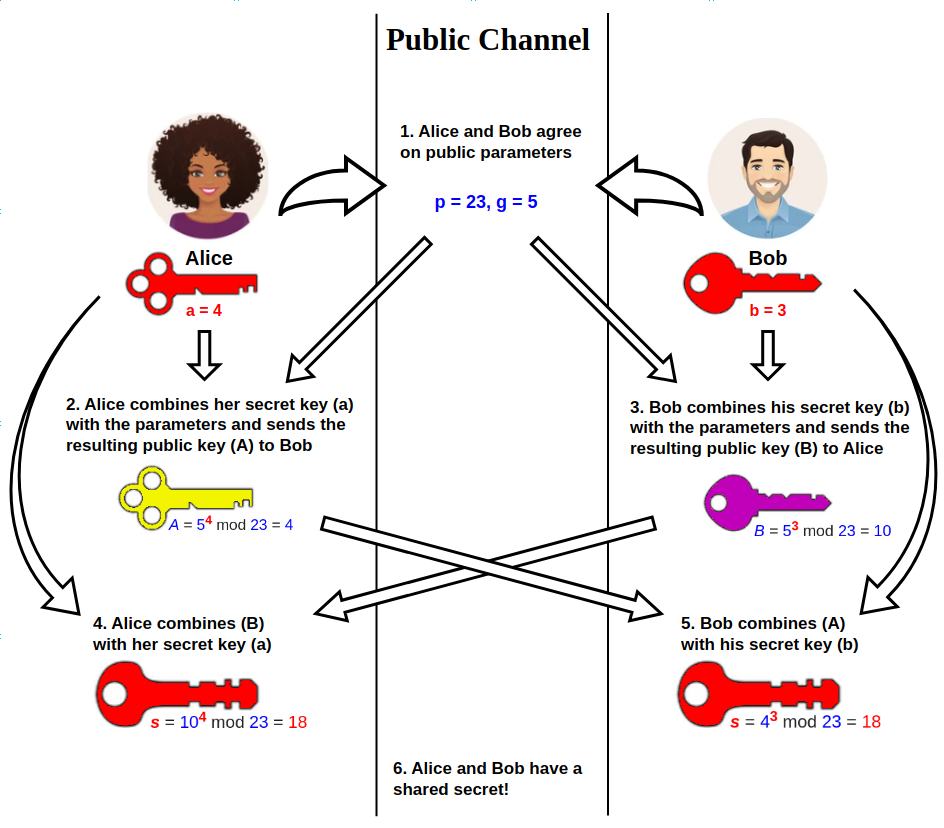
\includegraphics[width=8cm]{dh}
\end{frame}
% Źródła:
%   https://en.wikipedia.com/wiki/Diffie%E2%80%93Hellman_key_exchange
%

\begin{frame}{Secure Remote Password v6.a (SRP) (1)}
    \begin{definition}
        Protokół umożliwiający bezpieczne uwierzytelnienie jednej ze stron w drugim systemie.
    \end{definition}

    Założenia początkowe:
    \begin{itemize}
        \item $ q, N \in \mathbb{P} \land N \ge 1000 \text{ bit} \land N = 2\cdot q + 1 $ oraz $N$ \textbf{jest jawne},
        \item $ g\mod N$ stanowiący generator grupy multiplikatywnej modulo $N$ oraz $g$ \textbf{jest jawne},    %taka liczba, że jej potęgi generują wszystkie reszty modulo N%
        \item dysponujemy bezpieczną funkcja skrótu $hash(\cdot)$ ,
        \item $ k = hash(N, g) $,
        \item posiadamy dobre źródło losowości.
    \end{itemize}

    Uwaga: symbol $\oplus$ oznacza konkatenację.
    
\end{frame}
% Źródła:
    %   https://zaufanatrzeciastrona.pl/post/jak-blizzard-zabezpiecza-wasze-hasla-czyli-protokol-srp-i-czy-mozna-go-zlamac/
    %   http://srp.stanford.edu/design.html
    %   https://en.wikipedia.org/wiki/Secure_Remote_Password_protocol
    %   https://datatracker.ietf.org/doc/html/rfc2945
    %   https://pl.wikipedia.org/wiki/Grupa_cykliczna

\begin{frame}{Secure Remote Password v6.a (SRP) (2)}
    Tworzenie konta:
    \begin{enumerate}
        \item Klient wybiera login $I$ oraz hasło $P$, generuje losową sól $s$.
        \item Klient oblicza $x = hash(s \oplus hash(I \oplus \text{:} \oplus P))$ (zgodnie z RFC2945).
        \item Klient oblicza $v = g^{x} \bmod{N}$ i wysyła do serwera trójkę $(I, s, v)$. Należy też usunąć $x$ (tożsame z jawnym hasłem).
        \item Serwer zapisuje trójkę $(I, s, v)$ w swojej bazie danych użytkowników.
    \end{enumerate}
\end{frame}

\begin{frame}{Secure Remote Password v6.a (SRP) (3)}
    Weryfikacja:
    \begin{enumerate}
        \item Klient wysyła do serwera login $I$ oraz $A = g^{a} \bmod{N} \text{ gdzie } a \text { - losowe}$,
        \item Serwer wysyła do klienta sól $s$ oraz $B = (k\cdot v + g^{b} \bmod{N}) \text{ gdzie } b \text { - losowe}$.
        \item Obie strony obliczają wspólny sekret: $u = hash(A \oplus B)$.
        \item Klient oblicza: $S_{C} = (B - k\cdot g^{x})^{(a + u\cdot x)} \bmod{N}$.
        \item Serwer oblicza: $S_{S} = (A\cdot v^{u})^{b} \bmod{N}$.
        \item Obie strony obliczają klucz sesji: $ K_{C} = hash(S_{C})  \text{ , }  K_{S} = hash(S_{S}) $
        \item Klient wysyła do serwera dowód $M_{1} = hash( (hash(N) \text{ XOR } hash(g) ) \oplus hash(I) \oplus s \oplus A \oplus B \oplus K_{C})$.
        \item Serwer weryfikuje $M_{1}$ i wysyła do klienta dowód $M_{2} = hash(A \oplus M_{1} \oplus K_{S})$.
        \item Jeśli $M_{1} = M_{2}$, weryfikacja przebiegła poprawnie.
    \end{enumerate}
    
    Safeguards: 
    \begin{itemize}
        \item Przerywamy, jeśli:
            \begin{itemize}
                \item $B \equiv 0 \pmod{N}$ lub $u \equiv 0 \pmod{N}$ (klient),
                \item $A \equiv 0 \pmod{N}$ (serwer).
            \end{itemize} 
        \item Klient \textbf{pierwszy} wysyła swój dowód. Serwer ujawnia swój dowód, tylko gdy oba dowody zgadzają się.
    \end{itemize}
\end{frame}

\begin{frame}[allowframebreaks]{Źródła}
    \small
    \begin{thebibliography}{99}
        \bibitem{ref1} \url{https://mathworld.wolfram.com/ModularArithmetic.html}
        \bibitem{ref2} \url{https://simple.wikipedia.org/wiki/Modular_arithmetic}
        \bibitem{ref3} \url{https://archive.org/details/disquisitionesa00gaus/page/X/mode/2up}
        \bibitem{ref4} \url{https://view.fis.agh.edu.pl/staff/lenda/number_theory/A31.pdf}
        \bibitem{ref5} \url{https://pl.wikipedia.org/wiki/MaC582e_twierdzenie_Fermata}
        \bibitem{ref6} \url{https://deltami.edu.pl/2017/04/male-twierdzenie-fermata/0A}
        \bibitem{ref7} \url{https://pl.wikipedia.org/wiki/Funkcja_CF86}
        \bibitem{ref8} \url{https://en.wikipedia.org/wiki/Euler27s_theorem}
        \bibitem{ref9} \url{https://cp-algorithms.com/algebra/discrete-log.html}
        \bibitem{ref10} \url{https://fizyka.umk.pl/~gniewko/didaktiki/MD2013-2014/wykC582ad9.pdf}
        \bibitem{ref11} \url{https://en.wikipedia.org/wiki/Blum_Blum_Shub}
        \bibitem{ref12} \url{https://asecuritysite.com/encryption/blum}
        \bibitem{ref30} \url{https://www.researchgate.net/profile/Lenore-Blum/publication/221354947_Comparison_of_Two_Pseudo-Random_Number_Generators/links/00463531f2e378e090000000/Comparison-of-Two-Pseudo-Random-Number-Generators.pdf}
        \bibitem{ref13} \url{https://en.wikipedia.org/wiki/Luhn_algorithm}
        \bibitem{ref14} \url{http://www.algorytm.org/sumy-kontrolne/algorytm-luhna-mod-10.html}
        \bibitem{ref15} \url{https://en.wikipedia.org/wiki/Cyclic_redundancy_check}
        \bibitem{ref16} \url{https://pl.wikipedia.org/wiki/Cykliczny_kod_nadmiarowy}
        \bibitem{ref17} \url{https://ucgosu.pl/2017/01/jak-dziala-crc/}
        \bibitem{ref18} \url{https://www.geeksforgeeks.org/dsa/modulo-2-binary-division/}
        \bibitem{ref19} \url{https://en.wikipedia.org/wiki/RSA_cryptosystem}
        \bibitem{ref20} \url{https://eduinf.waw.pl/inf/utils/010_2010/0219.php}
        \bibitem{ref21} \url{https://en.wikipedia.org/wiki/DiffieE28093Hellman_key_exchange}
        \bibitem{ref22} \url{https://www.math.brown.edu/johsilve/MathCrypto/SampleSections.pdf}
        \bibitem{ref23} \url{https://www.geeksforgeeks.org/dsa/primitive-root-of-a-prime-number-n-modulo-n/}
        \bibitem{ref24} \url{https://en.wikipedia.com/wiki/DiffieE28093Hellman_key_exchange}
        \bibitem{ref25} \url{https://zaufanatrzeciastrona.pl/post/jak-blizzard-zabezpiecza-wasze-hasla-czyli-protokol-srp-i-czy-mozna-go-zlamac/}
        \bibitem{ref26} \url{http://srp.stanford.edu/design.html}
        \bibitem{ref27} \url{https://en.wikipedia.org/wiki/Secure_Remote_Password_protocol}
        \bibitem{ref28} \url{https://datatracker.ietf.org/doc/html/rfc2945}
        \bibitem{ref29} \url{https://pl.wikipedia.org/wiki/Grupa_cykliczna}
        
    \end{thebibliography}
\end{frame}

\end{document}
